
\subsection{その他}

\subsubsection{Probe 出力}


\begin{multicols}{2}
信号処理中の中間信号を取り出すための Probe 出力ラインがフロントパネルに用意されている。出力することができる中間信号を以下に示す。
\begin{itemize}
\item HighGain PreAmp 出力
\item LowGain PreAmp 出力
\item HighGain Slow shaper 出力
\item LowGain Slow shaper 出力
\item Fast shaper
\end{itemize}
前述の RegisterValue.yml から出力する情報を指定することができる。\\

PreAmp を選択した場合、波形全体ではなくピーク付近の一部のみ出力される。注意点としては、2 ch 以上を同時に ON にしない、データ取得中は Probe 1,2 を OFF にすること。


\begin{figure}[H]
\begin{center}
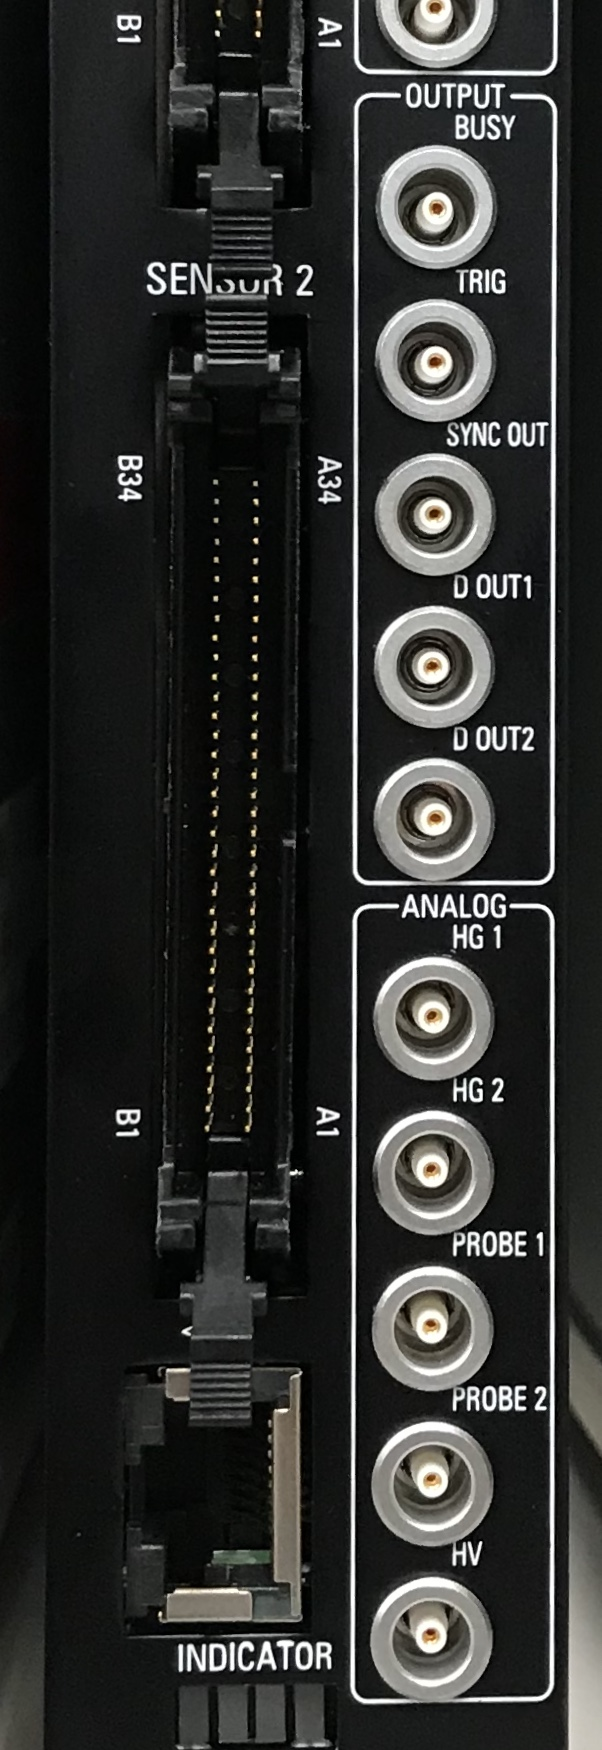
\includegraphics[width = 3cm, bb= 0 0 602 1750]{6.jpg}
\end{center}
\caption{フロントパネルの Probe 出力}
\label{fig:}
\end{figure}
\end{multicols}


\begin{shadebox}
\begin{verbatim}
High Gain Channel 1: 0   # HG で読み出すチャンネルの指定
High Gain Channel 2: -1  # 読み出すなら ch_#、読み出さないなら-1
Probe Channel 1: -1      # Probe からの出力チャンネル選択
Probe Channel 2: -1      # 2 ch 以上同時に使用しない
Probe 1: Out_PA_HG
Probe 2: Out_fs  # Out_PA_HG, Out_PA_LG, Out_ssh_HG, Out_ssh_LG, Out_fs
\end{verbatim}
\end{shadebox}
 \\
また、SYNC OUT からの周期信号も RegisterValue.yml より変更が可能である。

\begin{shadebox}
\begin{verbatim}
UsrClkOut: "OFF"  # "OFF", "ON", 1Hz, 10Hz, 100Hz, 1kHz, 10kHz, 100kHz, 3MHz, ...
\end{verbatim}
\end{shadebox}


\newpage
\subsubsection{横山研所有のEASIROC}
2019年5月9日現在、5つの EASIROC ボードの存在が確認された。うち一つは京大高エネルギー研究室の備品と思われる。IP アドレスは DAC との接続の際に必要となる。
\begin{table}[H]
\begin{center}
\caption{横山研所有のEASIROC}
\begin{tabular}{ccc} \hline
管理No. & IP Adress & 備考 \\ \hline
1 & 192.168.10.11 &  \\ 
2 & 192.168.10.12 &  \\ 
3 & 192.168.10.13 &  \\ 
2号 & 192.168.10.18 & ch.32 の読み出し不調。バイアス HV にふらつきあり。 \\ 
京大高エネ備品 & 不明 & 後半 32ch の InputDAC が動かない。連絡先:075-753-3837。  \\ \hline
\end{tabular}
\end{center}
\end{table}


\newpage
\section{参考文献}
1,2,3 は EASIROC 開発時の資料、4,5 はアップグレード後の資料である。
\begin{enumerate}
\item OpenIt のサイト\\
\url{http://openit.kek.jp/project/MPPC-Readout-Module/public/MPPC-Readout-Module}
\item 石島さんの修論\\
\url{http://osksn2.hep.sci.osaka-u.ac.jp/theses/master/2013/ishijima_mthesis.pdf}
\item 塩崎さんの修論\\
\url{http://lambda.phys.tohoku.ac.jp/~db/human_resource/thesis/2009_B_2_M_1.pdf}
\item 竹馬さんのマニュアル\\
\url{http://hep.phys.s.u-tokyo.ac.jp/~nchikuma/easiroc_manual.html} 
\item 竹馬さんの修論\\
\url{http://hep.phys.s.u-tokyo.ac.jp/wordpress/wp-content/uploads/2016/06/mth2016_chikuma.pdf}
\end{enumerate}

\end{document}



